\documentclass{beamer}

\usepackage{graphicx}
\usepackage[latin1]{inputenc}
\usepackage[T1]{fontenc}
\usepackage[english]{babel}
\usepackage{listings}
\usepackage{xcolor}
\usepackage{eso-pic}
\usepackage{mathrsfs}
\usepackage{url}
\usepackage{amssymb}
\usepackage{amsmath}
\usepackage{multirow}
\usepackage{hyperref}
\usepackage{booktabs}
% \usepackage{bbm}
\usepackage{cooltooltips}
\usepackage{colordef}
\usepackage{beamerdefs}
\usepackage{lvblisting}
\usepackage{setspace} % to be able to temporarily change "Zeilenabstand"
\usepackage{sansmathaccent} % to be able to use math without error
\pdfmapfile{+sansmathaccent.map}

\pgfdeclareimage[height=2cm]{logobig}{hulogo}
\pgfdeclareimage[height=0.7cm]{logosmall}{Figures/LOB_Logo}

\renewcommand{\titlescale}{1.0}
\renewcommand{\titlescale}{1.0}
\renewcommand{\leftcol}{0.6}

\title[Stacking Algorithm for Ensemble Modelling]{Stacking Algorithm for Ensemble Modelling}
\authora{Frederik Schreck}
\authorb{}
\authorc{}

\def\linka{}
\def\linkb{}
\def\linkc{}

\institute{Course: Numerical Introductory Course \\
Lecturer: Prof. Dr. Brenda L�pez Cabrera
Humboldt--Universit�t zu Berlin \\}

\hypersetup{pdfpagemode=FullScreen}

\begin{document}

% 0-1
%%%%%%%%%%%%%%%%%%%%%%%%%%%%%%%%%%%%%%%%
\frame[plain]{
\titlepage
}


%%%%%%%%%%%%%%%%%%%%%%%%%%%%%%%%%%%%%%%%
\section{Motivation}
%%%%%%%%%%%%%%%%%%%%%%%%%%%%%%%%%%%%%%%%

\frame{
\frametitle{Motivation - The wisdom of the crowd}
\begin{itemize}
\item The aggregation of individual guesses	 in groups is often superior to individual guesses - even to experts
\item BUT: Only fulfilled under certain criteria %\cite{Surowiecki:2005:WC:1095645}:
	\begin{itemize}
	\item Variation of guesses
	\item Independence of guesses
	\item Decentralization 
	\item Algorithm
	\end{itemize}
\end{itemize}
}

%TEXT: 
%Start with this story: In 1906, Francis Galton's went to a county fair, and attended an interesting contest. People were asked to guess the %weight of an ox. About 800 visitors of the fair gave a guess, but no one in the end got the exact result: 1.198 pounds. %However, when aggregating the individual guesses, the average was really close: 1,197 pounds. 

% The concept behind this is known as "wisdom of the cloud"

%	Independence of guesses = people decide independent from each other. Or only small correlation of individual guesses. I will come back later to this point.
% 	Decentralization = 	People are able to specialize and draw their knowledge (?); 
%	Algorithm = results clearly depend on whether mean or median or s.th. else

% Exactly, this is the motica

%%%%%%%%%%%%%

%%%%%%%%%%%%%%%%%%%%%%%%%%%%%%%%%%%%%%%%
\section{Outline}
%%%%%%%%%%%%%%%%%%%%%%%%%%%%%%%%%%%%%%%%

\frame{
\frametitle{Outline}

\begin{enumerate}
\item Motivation \quad \checkmark
\item Decision Tree
\item Ensemble Learning
\item Stacking algorithms
\begin{enumerate}
\item Bagging and Random Forest
\item Boosting and Gradient Boosting
\item Bayes??
\item Stacked Generalization
\end{enumerate}
\item Potentials and Problems of Ensemble Learning
\item The German Credit Dataset
\item Sources
\end{enumerate}
}



%%%%%%%%%%%%%%%%%%%%%%%%%%%%%%%%%%%%%%%%
\section{Decision Tree}
%%%%%%%%%%%%%%%%%%%%%%%%%%%%%%%%%%%%%%%%

\frame{
\frametitle{Decision Tree}
\begin{itemize}
\item Idea: use a set of splitting rules to recursively partition the dataset.
\item Classification trees:
\begin{itemize}
\item Minimize impurity within nodes
\end{itemize}
\item Regression trees:
\begin{itemize}
\item Minimize variance of the response variable within nodes
\end{itemize}
\end{itemize}
}
% Draw two pictures for classification tree: one twodimensional graph (x-axis = age, y-axis = wage; Dependente var = risky customer (YES/NO); draw some dots into graph and separate them by lines while explaining the tree. Second plot is the tree structure.--> Explain how tree is build. And then explain how tree is used for prediction of a new datapoint.)

%%%%%%%%%%%%%%%%%%%%%%%%%%%%%%%%%%%%%%%%
\section{Decision Tree}
%%%%%%%%%%%%%%%%%%%%%%%%%%%%%%%%%%%%%%%%
% Since I evaluate a classification task in my paper, I will here focus on classification tree (and later stacking models for classification tasks.)
\frame{
\frametitle{Decision Tree for classification}
\begin{itemize}
\item Choice of splitting rule: maximizing information gain (IG) by decreasing node impurity (I) 
\begin{flalign}
IG_n = I_n - p_{n_1} * I(n_1) - p_{n_2} * I(n_2),
\end{flalign}
for node $n$ with branching nodes $n_1$ and $n_2$, and $p_{n_i}$ as the fraction of cases in branching node $n_i$\\
\item How to measure impurity? Choices of splitting criteria:
\begin{flalign}
&\text{Entropy:} I(n) = -\sum_{j}^{J} p(c_j|n) * \log_{2}(p(c_j|n))\\
&\text{Gini impurity:} I(n) = 1 - \sum_{j}^{J} p(c_j|n)^2\\
&\text{Misclassification impurity:} I(n) = 1 - \max_{{j}}	p(c_j),
\end{flalign}
for classes $c_j, j \in J = \{1,2,...\}$
\end{itemize}
}

\frame{
\frametitle{Decision Tree for classification}
\begin{itemize}
\item Choice of stopping rule:\\
A fully grown tree has pure leaf nodes and may overfit the data\\
However, a too small tree may not capture all relevant structure of the data
\begin{itemize}
\item Pre-pruning
\item Post-pruning
\end{itemize}
\end{itemize}
}
%prepruning means to not grow tree fully but stop earlier-->Choice of stopping criteria (e.g. maximal depth)
%postpruning means to first fully grow the tree, and then cut the branches that are less important w.r.t. e.g. the decrease of impurity. For that we use new data.
%--> Decision trees are prone to overfitting. We can however correct for this by the methods I will introduce you to later.


%%%%%%%%%%%%%%%%%%%%%%%%%%%%%%%%%%%%%%%%
\section{Ensemble Learning}
%%%%%%%%%%%%%%%%%%%%%%%%%%%%%%%%%%%%%%%%

\frame{
\frametitle{Ensemble Learning - Terminology}
Machine Learning
\begin{itemize}
\item Part of computer science that uses statistical techniques to train models on data
\item Typically used for prediction purposes
\end{itemize}
\vspace{0.5cm}
Stacking and Ensemble Learning
\begin{itemize}
\item Idea is to combine hypotheses of multiple learning algorithms (base learners)
% explain word "hypothesis". So we combine the base learners' hypotheses in order to get a new hypothesis. Finite set of base learners used. 
\item Goal is to obtain a better predictive performance than with each of the single algorithms alone
\item Mainly used in supervised learning
% There have been some applications in unsupervised models, like for example "consensus clustering" but in general ensembling focuses on supervised learning.
\item Very flexible method
% The ensembling hypothesis, however, is not necessarily contained within the hypothesis space of the models from which it is built.Ensembles can be shown to have more flexibility in the functions they can represent.
\end{itemize}
}


\frame{
\frametitle{Ensemble Learning}
Which models to combine?
\begin{itemize}
\item Effective ensembling builds on diverse and little correlated models %\cite{kuncheva2003measures}
\item Best to use strong base learners
% Research has been shown that ensembling is most effective when base learners already have good predictions.
% SO, we see the same criteria than I mentioned in the motivation of this presentation! Also clearly the choice of algorithm is important. In the next sections, I will introduce different stacking models in ensemble modelling. But first, for all of you to be able to follow, I want to shortly explain the concept behind Decisions Trees, since Trees are very often chosen ase base learners in ensemble models.
\end{itemize}
\vspace{0.5cm}
Similar criteria as mentioned in the Motivation!
}

\frame{
\frametitle{Ensemble Learning}
Which models to combine?
\begin{figure}[htb]
	\begin{center}
	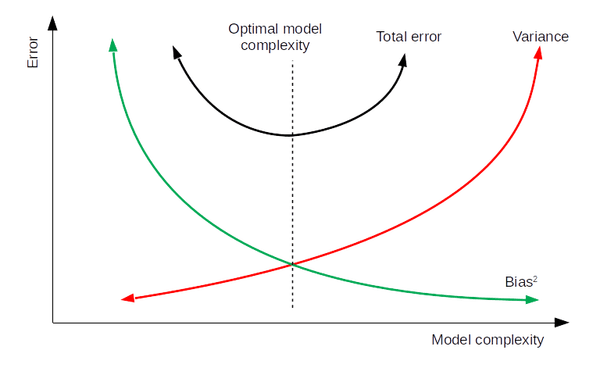
\includegraphics[scale=0.38, trim={0.5cm 1.3cm 0 0}]{Figures/bias_variance_tradeoff.png}
	\caption{The bias-variance-trade-off.}
	\end{center}
\end{figure}
\begin{itemize}
\item Combining complex classifiers may reduce variance.
% e.g. averaging over many estimates gives more robust estimation
\item Combining simple classifiers may reduce bias.
% combining simple rules gives eventually a complex rule
\end{itemize}
}


%%%%%%%%%%%%%%%%%%%%%%%%%%%%%%%%%%%%%%%%
\section{Bagging and Random Forest}
%%%%%%%%%%%%%%%%%%%%%%%%%%%%%%%%%%%%%%%%

\frame{
\frametitle{Bagging (= Bootstrap Aggregating)}
\begin{itemize}
\item Proposed by Leo Breiman %\cite{breiman1996bagging}
\item Meta-algorithm, designed to
\begin{itemize}
\item improve accuracy of base algorithms
\item reduce MSE by reducing variance % bias is not changed due to bagging
\item avoid overfitting problems
\item obtain smoother prediction boundaries
% possibly draw a two dimensional coordinate system with two features as axes and two colored dots (group 1 as a circle). Then draw lines from different (small) trees and show that by drawing many lines, the prediction boundary becomes smooth.
\end{itemize} 
\item Can be applied to all kinds of base learners
\item However best to use unstable methods that tend to have high variance, like trees
\end{itemize}
}

\frame{
\frametitle{Bagging algorithm}
\rule{10cm}{0.05cm}\\
for base learner $m$ in $\{1,2,...,M\}$\\
\hspace{1cm}uniformly draw sample $D_m$ with size $N$ from dataset $D$ \\\hspace{1cm}(with replacement)\\
\hspace{1cm}build model $T_m$ on dataset $D_m$\\
combine hypotheses 

\rule{10cm}{0.05cm}\\
\begin{itemize}
\item Combining by averaging in regression problems
\item Combining by majority vote in classification problems
\end{itemize}
}


\frame{
\frametitle{Random Forest}
\begin{itemize}
\item Also proposed by Leo Breiman %\cite{breiman2001random}
\item Random forests combine bagging with random subspace approach % \cite{ho1998random}
\item Random subspace randomly samples features from set of all features for each learner (with replacement)
\begin{itemize}
\item Reduces the correlation between estimators
\item Thus decreases variance in the ensemble learner
\end{itemize}
\item Random feature sampling happens at tree level or at split level
\item Random Forest only possible with tree-based base learners
\end{itemize}
}

\frame{
\frametitle{Random Forest algorithm for classification}
\rule{10cm}{0.05cm}\\
for base learner $m$ in $\{1,2,...,M\}$\\
\hspace{1cm}uniformly draw sample $k_m$ of size $L$ from features $\{1,2,...,K\}$ \\\hspace{1cm}(with replacement)\\
\hspace{1cm}uniformly draw sample $D_m$ with size $N$ from dataset $D$ \\\hspace{1cm}(with replacement)\\
\hspace{1cm}build model $T_{m}$ on dataset $D_m$ with feature set $k_m$ \\
$\hat{C}_{rf}^{L,N}(x) = \text{majority vote}\{\hat{T}_{m}\}_{1}^{M}$
\rule{10cm}{0.05cm}\\
}
% which are the tunable parameters: number of trees (the more the better, but computational costs increase), number of features for each tree, bootstrap sample sizes, number of branches for trees OR other sort of pruning...


\frame{
\frametitle{Random Forest algorithm for classification}
Random Forest vs. single Tree\\
\begin{table}
\centering
\begin{tabular}{p{.48\textwidth}|p{0.45\textwidth}}
Random Forest & Single Tree \\
\hline
\begin{itemize}
\item[$-$] higher computational costs %lot of storage memory and time
\item[$-$] blackbox %but importanceplots
\item[$+$] easy to tune parameters
\item[$+$] smaller prediction variance % so better performance
\item[$+$] scalability
\item[$-$] many parameter choices to make
\end{itemize}
&
\begin{itemize}
\item[$+$] computationally simple
\item[$+$] insights into decision rules
\item[$+$] easy to tune parameters
\item[$-$] tend to overfit and have high variance
\end{itemize}
\end{tabular}
\end{table}
}


%%%%%%%%%%%%%%%%%%%%%%%%%%%%%%%%%%%%%%%%
\section{Boosting and Gradient Boosting}
%%%%%%%%%%%%%%%%%%%%%%%%%%%%%%%%%%%%%%%%

\frame{
\frametitle{Boosting}

}


\frame{
\frametitle{Gradient Boosting}

}


%%%%%%%%%%%%%%%%%%%%%%%%%%%%%%%%%%%%%%%%
\section{Bayes??}
%%%%%%%%%%%%%%%%%%%%%%%%%%%%%%%%%%%%%%%%

\frame{
\frametitle{Bayes??}

}

%%%%%%%%%%%%%%%%%%%%%%%%%%%%%%%%%%%%%%%%
\section{Stacked Generalization}
%%%%%%%%%%%%%%%%%%%%%%%%%%%%%%%%%%%%%%%%

\frame{
\frametitle{Stacked Generalization}

}

%%%%%%%%%%%%%%%%%%%%%%%%%%%%%%%%%%%%%%%%
\section{Potentials and Problems of Ensemble Learning}
%%%%%%%%%%%%%%%%%%%%%%%%%%%%%%%%%%%%%%%%

\frame{
\frametitle{Potentials of Ensemble Learning}
\begin{figure}[htb]
	\begin{center}
	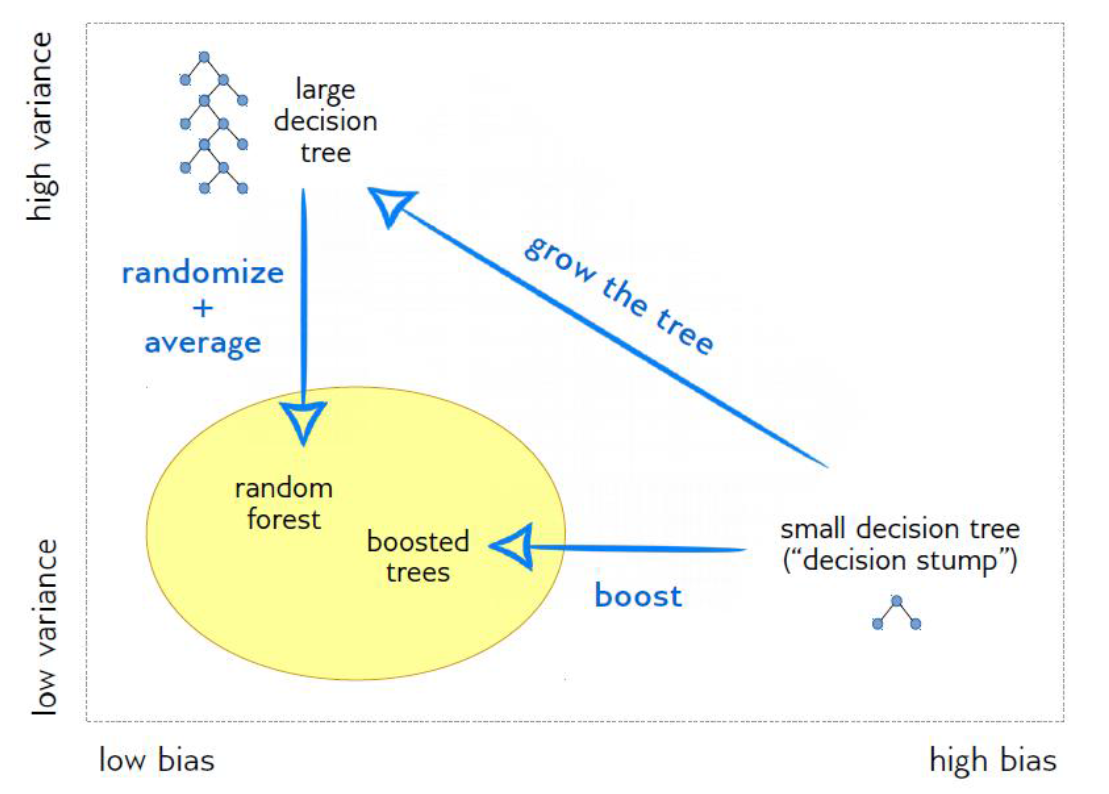
\includegraphics[scale=0.27, trim={0cm 1cm 0 0.5cm}]{Figures/bvtradeoff_boosting_bagging.png}
	\caption{How Gradient Boosting and Random Forest improve performance.}
	\end{center}
\end{figure}
}

\frame{
\frametitle{Problems of Ensemble Learning}

}


%%%%%%%%%%%%%%%%%%%%%%%%%%%%%%%%%%%%%%%%
\section{Sources}
%%%%%%%%%%%%%%%%%%%%%%%%%%%%%%%%%%%%%%%%

\frame{
\frametitle{Sources}
\bibliographystyle{apa}
\bibliography{library}
}

%%%%%%%%%%%%%%%%%%%%%%%%%%%%%%%%%%%%%%%%
\end{document}
